% Conceptual control groups, not a second rendering of the module UI.
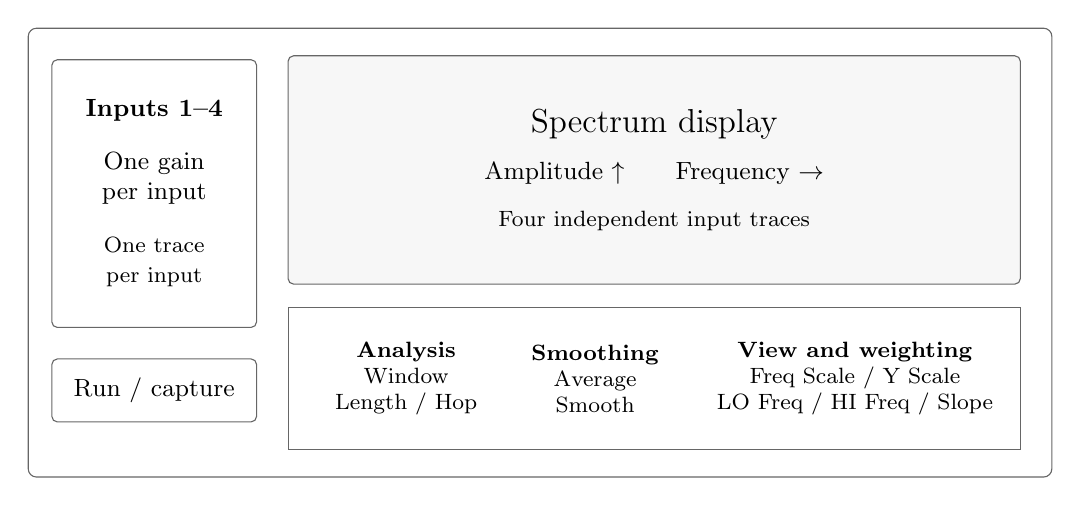
\begin{tikzpicture}[x=1cm,y=1cm,font=\small,
    region/.style={draw=black!60,rounded corners=2pt,align=center},
    label/.style={font=\footnotesize,align=center}]
  \draw[black!60,rounded corners=3pt] (0,0) rectangle (13,5.7);
  \node[region,minimum width=2.6cm,minimum height=3.4cm] at (1.6,3.6)
    {\textbf{Inputs 1--4}\\[8pt]One gain\\per input\\[8pt]
      \footnotesize One trace\\\footnotesize per input};
  \node[region,minimum width=2.6cm,minimum height=.8cm] at (1.6,1.1)
    {Run / capture};
  \node[region,fill=black!3,minimum width=9.3cm,minimum height=2.9cm]
    at (7.95,3.9) {\large Spectrum display\\[6pt]
      Amplitude $\uparrow$\qquad Frequency $\rightarrow$\\[6pt]
      \footnotesize Four independent input traces};
  \draw[black!60] (3.3,.35) rectangle (12.6,2.15);
  \node[label] at (4.8,1.25) {\textbf{Analysis}\\Window\\Length / Hop};
  \node[label] at (7.2,1.25) {\textbf{Smoothing}\\Average\\Smooth};
  \node[label] at (10.5,1.25) {\textbf{View and weighting}\\Freq Scale / Y Scale\\LO Freq / HI Freq / Slope};
\end{tikzpicture}
